\section{Diagramas UML: Modelagem Visual do Sistema}

\subsection{Diagrama de Casos de Uso}

O diagrama de casos de uso representa as funcionalidades do sistema do ponto de vista do usuário, demonstrando as interações entre os atores e os principais recursos disponíveis na plataforma.

\begin{figure}[H]
\centering
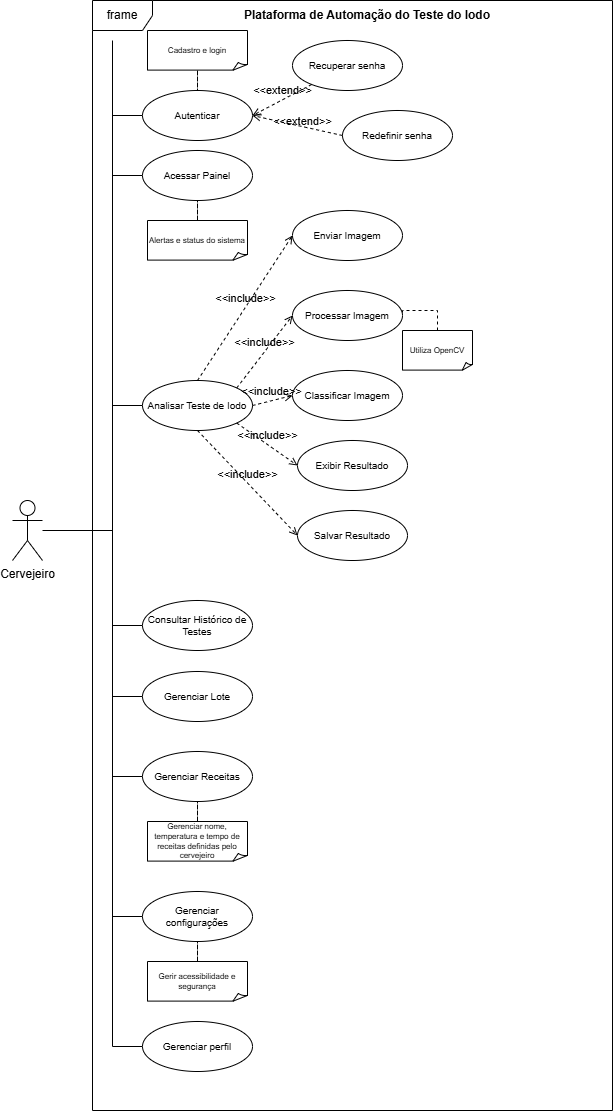
\includegraphics[height=0.9\textheight, keepaspectratio]{imgs/caso-de-uso.png}
\caption{Diagrama de Casos de Uso}
\label{fig:caso-de-uso}
\end{figure}

\subsection{Diagrama de Classes}

O diagrama de classes mostra a estrutura estática do sistema:

\begin{figure}[H]
\centering
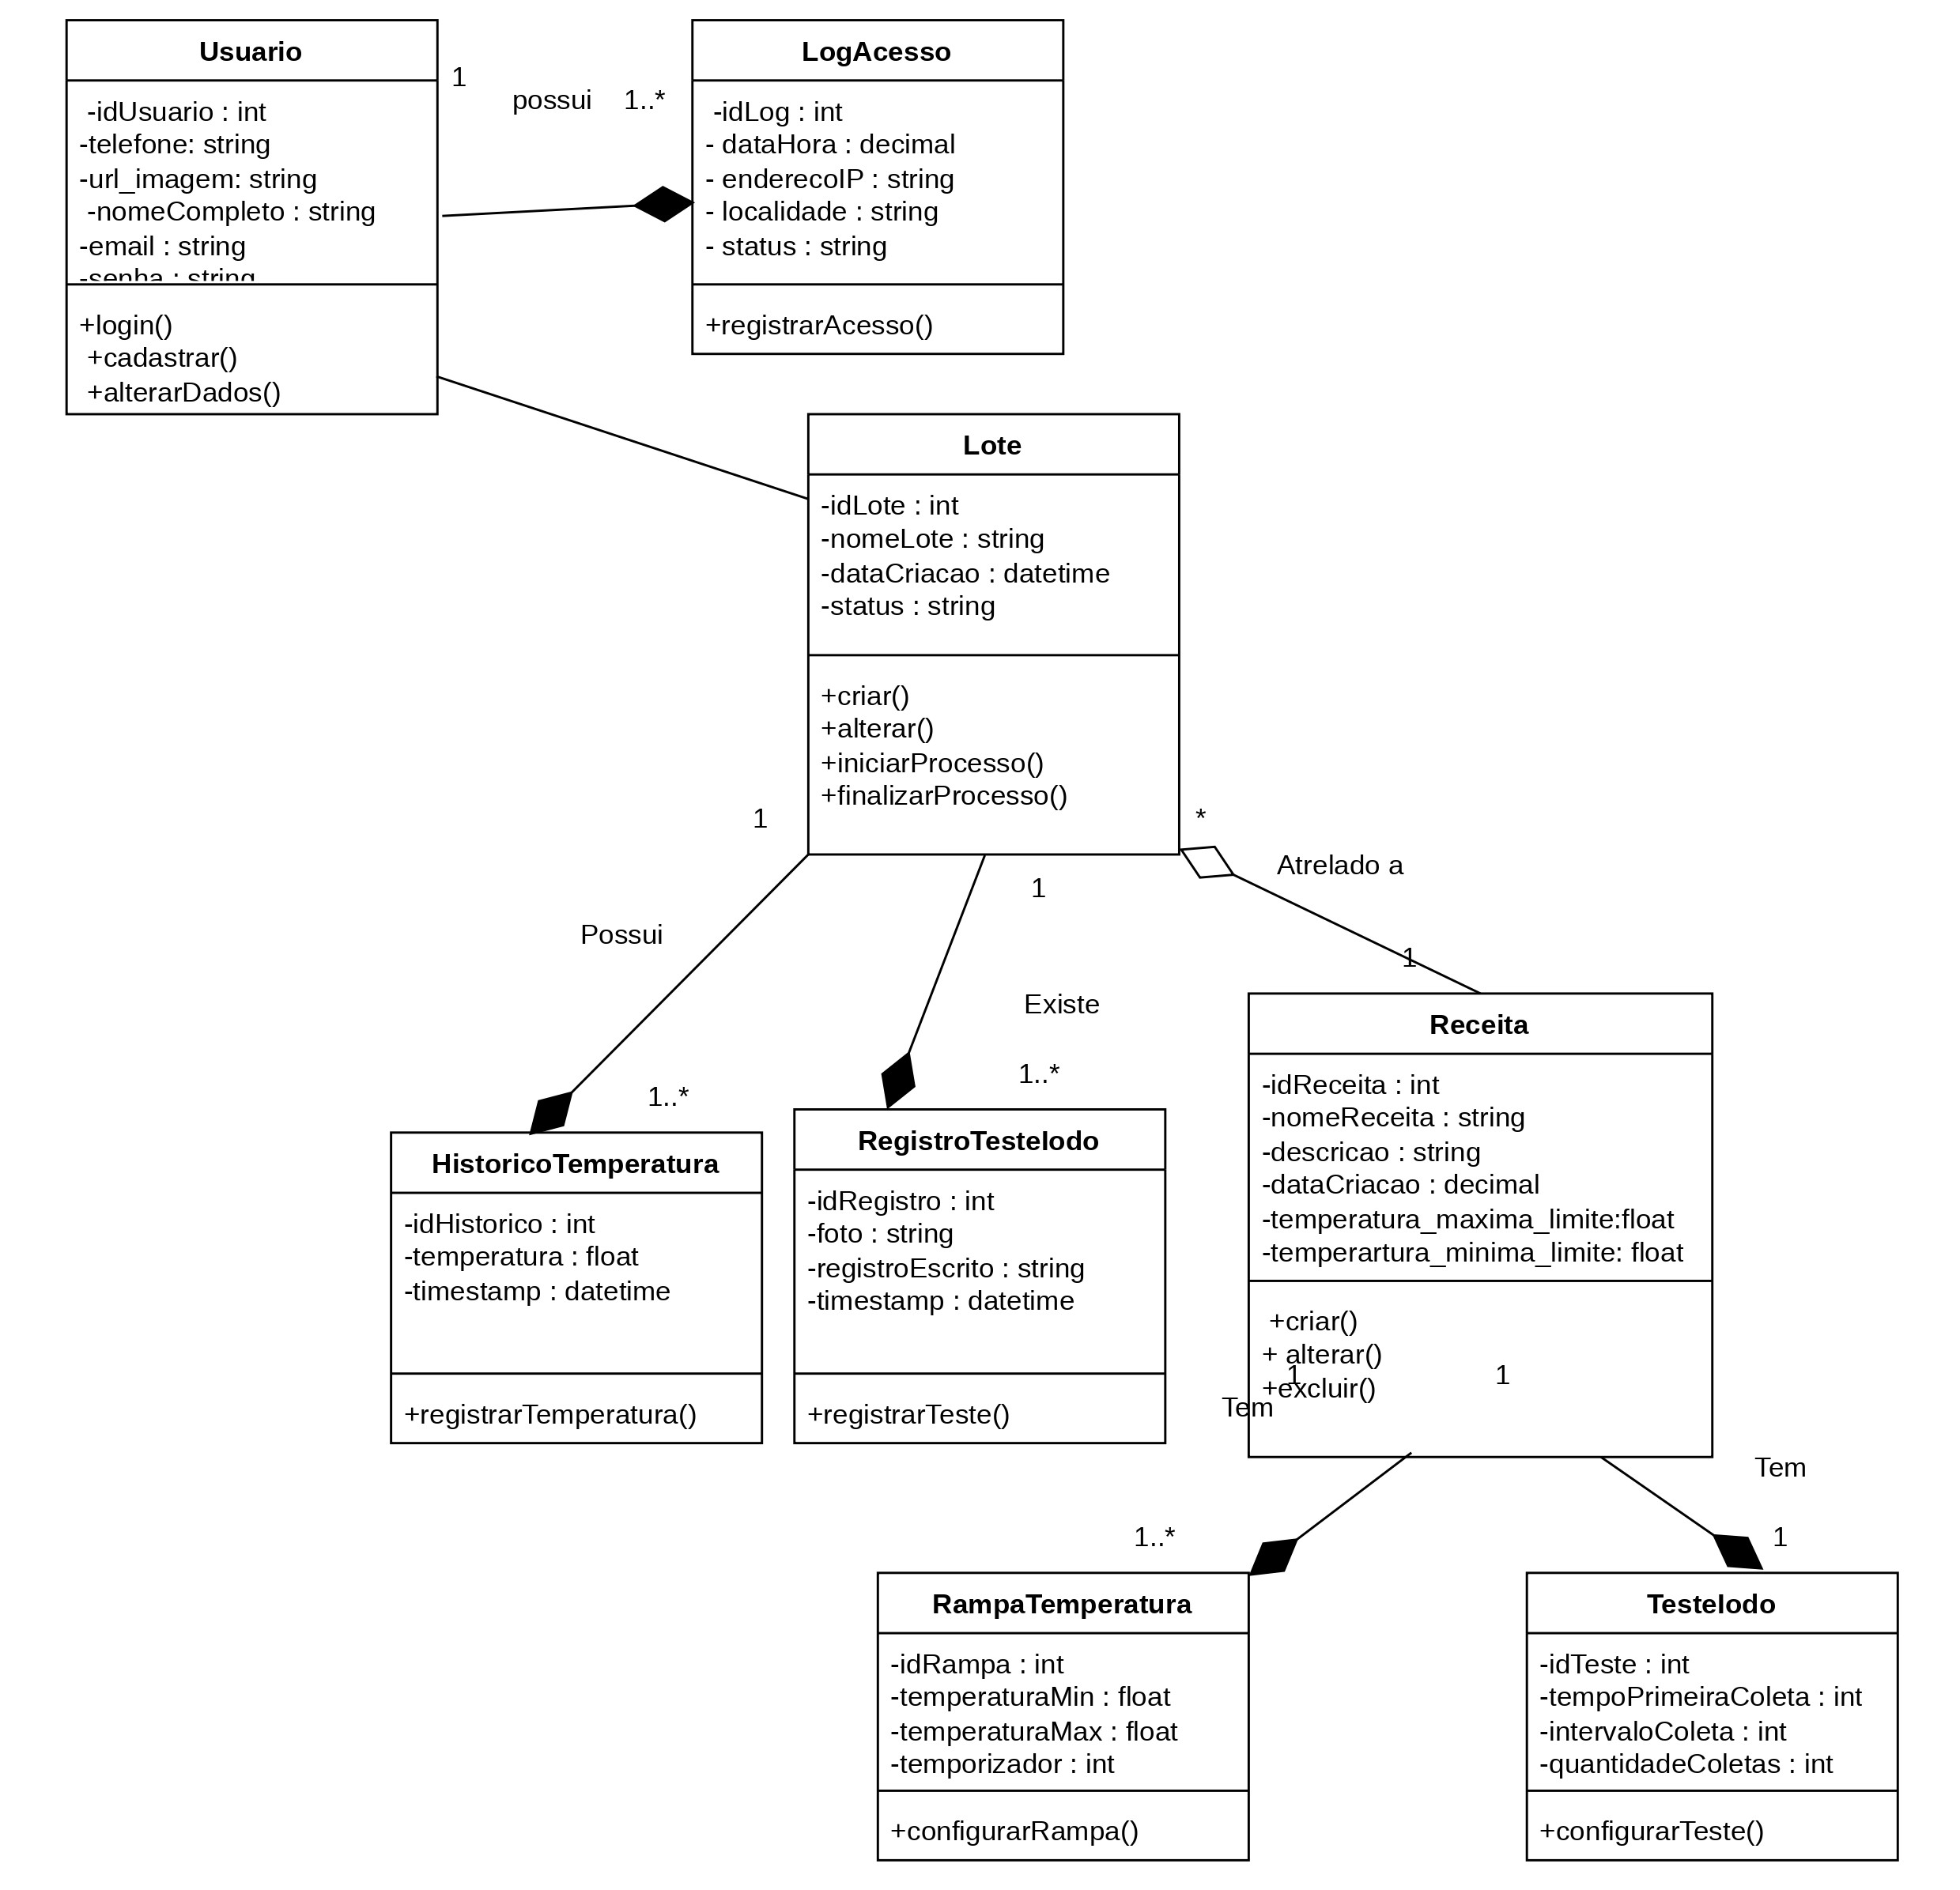
\includegraphics[width=\textwidth]{imgs/diagrama-de-classes.jpg}
\caption{Diagrama de Classes}
\label{fig:diagrama-de-classes}
\end{figure}

\subsection{Diagrama de Objetos}

O diagrama de objetos representa instâncias reais das classes utilizadas no sistema em um determinado momento da execução da aplicação. O diagrama de objetos demonstra exemplos concretos dos dados manipulados pela plataforma.

\begin{figure}[H]
\centering
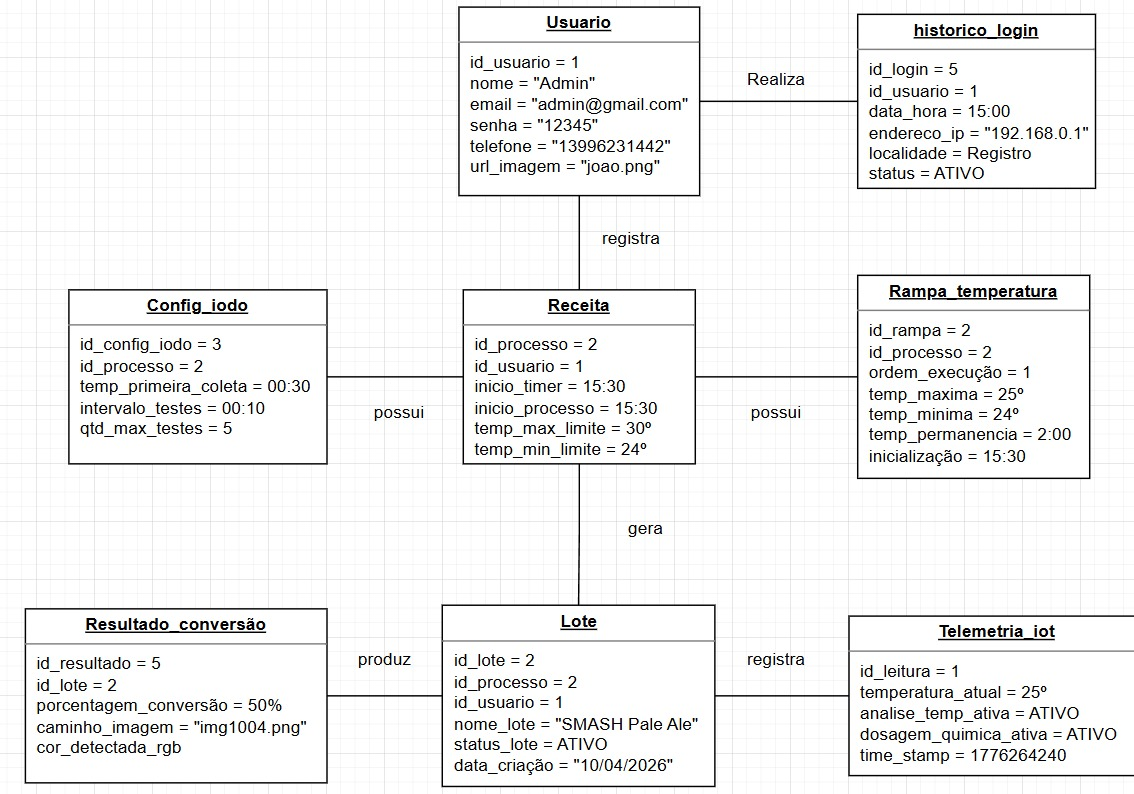
\includegraphics[width=0.9\linewidth]{imgs/diagrama-de-objetos.jpeg}
\caption{Diagrama de Objetos}
\label{fig:diagrama-objetos}
\end{figure}